\section{Introduction to sets}
   \subsection{} \{\ldots $-16,-11,-6,-1,4,9,14,$\ldots \}.
   \subsection{} \{\ldots $-7,-4,-1,2,5,8,11,$\ldots \}.
   \subsection{} \{$-2,-1,\ldots,6$\}.
   \subsection{} \{$1,2,\ldots,7$\}.
   \subsection{} \{$\pm\sqrt{3}$\}.
   \subsection{} \{$\pm 3$\}.
   \subsection{} \{$-2,-3$\}.
   \subsection{} \{$0,-2,-3$\}.
   \subsection{} $\mathbb{Z}$.
   \subsection{} \{$2\pi x : x \in \mathbb{Z}$\}.
   \subsection{} $\{-4,-3,\ldots,4\}$.
   \subsection{} $\{-2,-1,\ldots,2\}$.
   \subsection{} $\{0\}$.
   \subsection{} $\{-20,-15,-10,\ldots,10,15,20\}$.
   \subsection{} Let's call the set $S$. It's clear that every member of $S$ is
   an integer. Conversely, note that $n=5n+2(-2n)$, $n \in \mathbb{Z}$. Therefore,
   $S=\integerset$.
   \subsection{} The reasoning is similar, but note that there exists no $a,b \in \integerset$
   such that either $n=6n+2b$ or $n=6a+2b$, $n \in \integerset$. Also, note that
   $6a+2b=2(3a+b)$, in which $n=3n-2n$. Therefore, $S$ is the set of even integers in $\integerset$.
   \begin{equation}
     S = \{2n: n \in \integerset\} \subset \integerset
   \end{equation}

   \subsection{} $\{2^n: n\in\naturalset\}$.
   \subsection{Unsolved} Observation: Successive difference of each couple of
   numbers: $4, 12, 20, 28, 36,\ldots$ (a difference of 8 each).
   \subsection{} $\{3n: n \in \integerset\}$.
   \subsection{} $\{5n+2: n \in \integerset\}$.
   \subsection{} $\{n^2: n \in \integerset\}$.
   \subsection{Unsolved}
   My first conjecture was $2^n + n$, but it is wrong for the fourth number.
   \subsection{} $\{n \in \naturalset: 3 \leq n \leq 8\}$.
   \subsection{} $\{n \in \integerset: -4 \leq n \leq 2\}$.
   \subsection{} \set{2^n: n \in \integerset}.
   \subsection{} \set{3^n: n \in \integerset}.
   \subsection{} \set{\dfrac{n\pi}{2}: n \in \integerset}.
   \subsection{} \set{\dfrac{3}{4}n: n \in \integerset}.
   \subsection{} $3$. Namely, \set{1}, \set{2,\set{3,4}}, $\emptyset$.
   \subsection{} $5$. Namely, \set{1,4}, $a$, $b$, \set{\set{3,4}}, \set{\emptyset}.
   \subsection{} $1$. Namely, the biggest set that includes all the others.
   \subsection{} $1$. Same as above.
   \subsection{} $19$. Namely, $-9,-8,\ldots,8,9$.
   \subsection{} $9$. Namely, $1,\ldots,9$.
   \subsection{} $7$. Namely, $-3,\ldots,3$.
   \subsection{} $3$. Namely, $1,2,3$.
   \subsection{} $0$. Namely, $\emptyset$.
   \subsection{} $4$. Namely, $1,2,3,4$.

   \subsection{}
   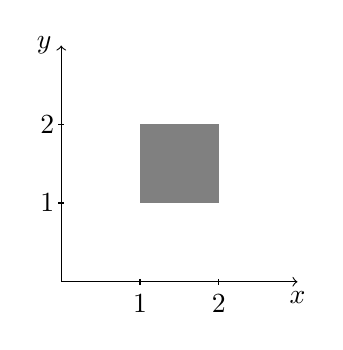
\begin{tikzpicture}
     \draw[<->] (0,3) node[left]{$y$} -- (0,0) -- (3,0) node[below]{$x$};
     \foreach \x in {1,2}
       \draw (\x,1pt) -- (\x,-1pt) node[below]{$\x$};
     \foreach \y in {1,2}
       \draw (-1pt,\y) -- (1pt,\y) node[left]{$\y$};
     \fill[fill=gray] (1,1) -- +(0,1) -- +(1,1) -- +(1,0) -- cycle;
   \end{tikzpicture}

   \subsection{}
   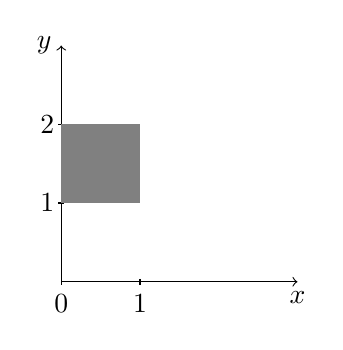
\begin{tikzpicture}
     \draw[<->] (0,3) node[left]{$y$} -- (0,0) -- (3,0) node[below]{$x$};
     \foreach \x in {0,1}
       \draw (\x,1pt) -- (\x,-1pt) node[below]{$\x$};
     \foreach \y in {1,2}
       \draw (-1pt,\y) -- (1pt,\y) node[left]{$\y$};
     \fill[fill=gray] (0,1) -- +(0,1) -- +(1,1) -- +(1,0) -- cycle;
   \end{tikzpicture}

   \subsection{}
   \begin{tikzpicture}
     \draw[->] (-2,0) -- (2,0) node[below]{$x$};
     \draw[->] (0,0) -- (0,2) node[left]{$y$};
     \foreach \x in {-1,0,1}
       \draw (\x,-1pt) -- (\x,1pt) node[below]{$\x$};
     \draw (-1pt,1) -- (1pt,1) node[above left]{$1$};
     \draw[gray] (-1,1) -- ++(2,0);
   \end{tikzpicture}

   \subsection{}
   \begin{tikzpicture}
     \draw[->] (-3,0) -- (3,0) node[below]{$x$};
     \draw[->] (0,0) -- (0,2) node[left]{$y$};
     \foreach \y in {0,1}
       \draw (-1pt,\y) -- (1pt,\y) node[above left]{$\y$};
     \draw (2,-1pt) -- (2,1pt) node[below]{$2$};
     \draw[thick,gray] (2,0) -- ++(0,1);
   \end{tikzpicture}

   \subsection{}
   \begin{tikzpicture}
     \draw[->] (-3,0) -- (3,0) node[below]{$x$};
     \draw[->] (0,0) -- (0,2) node[left]{$y$};
     \foreach \y in {0,1}
       \draw (-1pt,\y) -- (1pt,\y) node[above left]{$\y$};
     \foreach \x in {-2,2}
       \draw (\x,-1pt) -- (\x,1pt) node[below]{$\x$};
     \draw[thick,gray] (2,0) -- ++(0,1);
     \draw[thick,gray] (-2,0) -- ++(0,1);
   \end{tikzpicture}

   \subsection{}
   \begin{tikzpicture}[domain=-2:2,label/.style={postaction={decorate,%
     decoration={%
     markings,%
     mark = at position .75 with \node #1; }}}%
     ]
     \draw[->] (-3,0) -- (3,0) node[below]{$x$};
     \draw[->] (0,0) -- (0,5) node[left]{$y$};

     \draw[thick,gray,label={[above left]{$y=x^2$}}] plot(\x,\x*\x);
   \end{tikzpicture}

   \subsection{}
   \begin{tikzpicture}[domain=-1:1,label/.style={postaction={decorate,%
     decoration={%
     markings,
     mark = at position .95 with \node #1;}}}]
     \draw[->] (-3,0) -- (3,0) node[below]{$x$};
     \draw[->] (0,-3) -- (0,3) node[left]{$y$};

     \draw[thick,gray,label={[above right]{$x^2+y^2=1$}}] plot(\x,{sqrt(1-((\x)*(\x)))});
     \draw[thick,gray] plot(\x,{-sqrt(1-((\x)*(\x)))});
   \end{tikzpicture}

   \subsection{}
   \begin{tikzpicture}[domain=-1:1,label/.style={postaction={decorate,%
       decoration={%
       markings,
       mark = at position .95 with \node #1;}}}]
       \draw[->] (-3,0) -- (3,0) node[below]{$x$};
       \draw[->] (0,-3) -- (0,3) node[left]{$y$};

       \fill[thick,gray,label={[above right]{$x^2+y^2<=1$}}] plot(\x,{sqrt(1-((\x)*(\x)))});
       \fill[thick,gray] plot(\x,{-sqrt(1-((\x)*(\x)))});

   \end{tikzpicture}

   \subsection{}
   \begin{tikzpicture}[domain=-2:2,label/.style={postaction={decorate,%
     decoration={%
     markings,%
     mark = at position .75 with \node #1; }}}%
     ]
     \draw[->] (-3,0) -- (3,0) node[below]{$x$};
     \draw[->] (0,0) -- (0,5) node[left]{$y$};

     \fill[thick,gray,label={[above right]{$y \geq x^2-1$}}] plot(\x,{(\x)*(\x) - 1});
   \end{tikzpicture}

   \subsection{}
   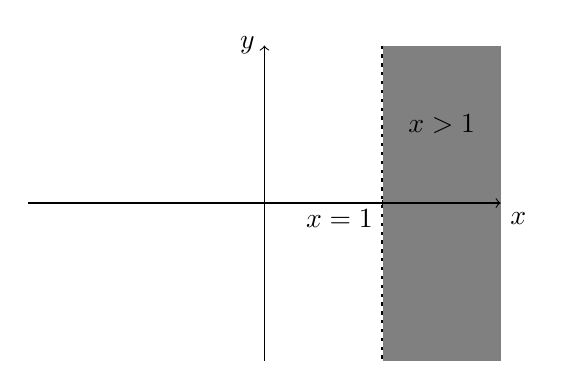
\begin{tikzpicture}[domain=-2:2,xscale=1.5]
     \draw[->] (0,-2) -- (0,2) node[left]{$y$};
     \draw (1,-1pt) -- (1,1pt) node[below left]{$x=1$};
     \draw[very thick,dotted] (1,2) -| (1,-2);
     \fill[gray] (1,2)--(2,2)--(2,-2)--(1,-2);
     \draw[->] (-2,0) -- (2,0) node[below right]{$x$};
     \draw (1.5,1) node{$x>1$};
   \end{tikzpicture}

   \subsection{}
   \begin{tikzpicture}[domain=-2:2,label/.style={postaction={decorate,
     decoration={
     markings,
     mark= at position .95 with \node #1;
     }}}]
     \draw[->] (0,-2) -- (0,2) node[left]{$y$};
     \draw[->] (-2,0) -- (2,0) node[below]{$x$};
     \draw[gray,label={[above]{$x+0$}}] plot(\x,\x);
     \draw (1,0.5) node{\vdots};
     \draw (1,1.5) node{\vdots};
     \draw[gray,label={[above]{$x+y$}}] plot(\x,{\x + 1});
     \draw[gray,label={[above]{$x+y$}}] plot(\x,{\x - 1});
   \end{tikzpicture}

   \subsection{}
   \begin{tikzpicture}[domain=-2:2,label/.style={postaction={decorate,
     decoration={
     markings,
     mark= at position 0.99 with \node #1;
     }}}]
     \draw[->] (0,-2) -- (0,2) node[left]{$y$};
     \draw[->] (-2,0) -- (2,0) node[below]{$x$};
     \draw[gray,label={[above right]{$x^2$}}] plot(\x,{(\x)*(\x)});
     \draw (2,0.5) node{\ldots};
     \draw[gray,label={[above right]{$\dfrac{x^2}{2}$}}] plot(\x,{((\x)*(\x)) / 2});
     \draw[gray,label={[right]{$\dfrac{x^2}{3}$}}] plot(\x,{((\x)*(\x)) / 3});
   \end{tikzpicture}

   \subsection{}
   \begin{tikzpicture}[domain=-2:2,label/.style={postaction={decorate,
     decoration={
     markings,
     mark= at position .95 with \node #1;
     }}}]
     \draw[->] (0,-2) -- (0,2) node[left]{$y$};
     \draw[->] (-2,0) -- (2,0) node[below]{$x$};
     \draw[gray,label={[above]{$y=x$}}] plot(\x,\x);
     \draw[gray,label={[above right]{$y=-x$}}] plot(\x,{-(\x)});
   \end{tikzpicture}

   \subsection{}
   \begin{tikzpicture}[domain=-2:2,label/.style={postaction={decorate,
     decoration={
     markings,
     mark= at position .95 with \node #1;
     }}}]
     \draw[->] (0,-2) -- (0,2) node[left]{$y$};
     \draw[->] (-2,0) -- (2,0) node[below]{$x$};
     \draw[gray,label={[above left]{$y=x^2$}}] plot(\x,{(\x) * (\x)});
     \draw[gray,label={[above right]{$y=-x^2$}}] plot(\x,{-(\x) * (\x)});
   \end{tikzpicture}

\clearpage
